\subsection{Visualizing Idle System Traces}
\label{sec:idle}

\begin{figure*}[htb]
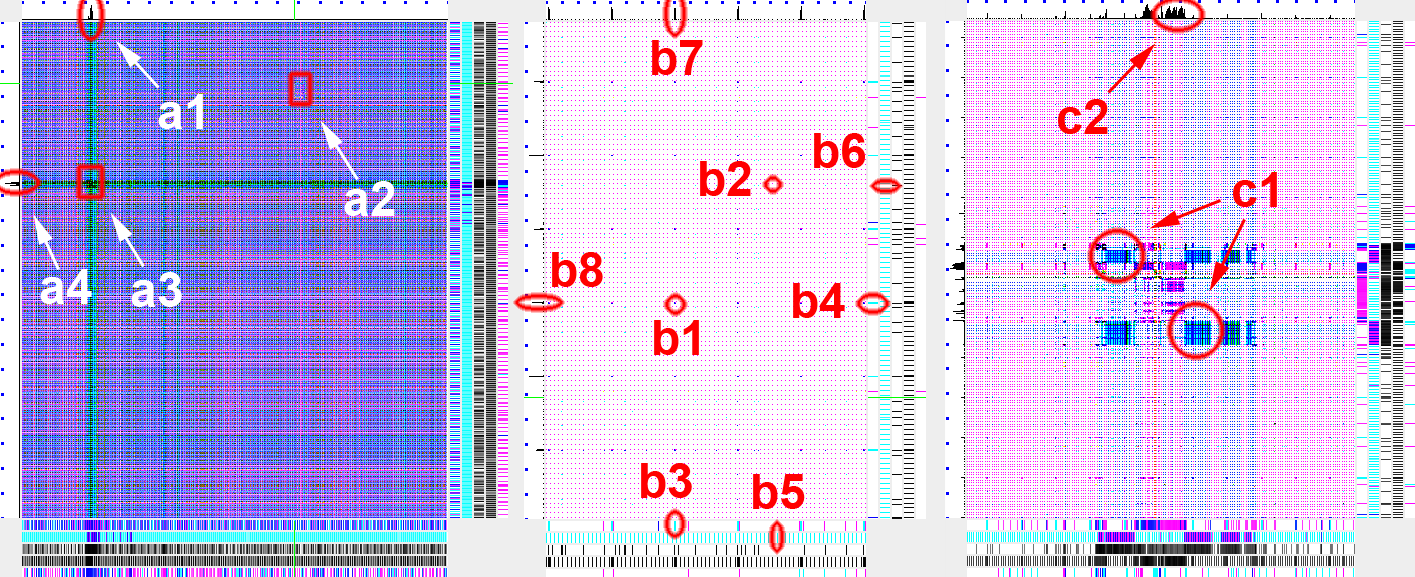
\includegraphics[width=1.0\textwidth]{lviz/idle-dp.png}
\caption{Time-ordered \VDP{} comparing two idle systems.
{\bf a.} (left) comparing one hour interval between two machines;
{\bf b.} (middle) zoom in of Region {\em a2};
{\bf c.} (right) zoom in of {\em a3}.
%DP Matching: (program,operation);
%DP color: file=cyan, registry=magenta, other operation=yellow;
%Bar1: lsass.exe=cyan, svchost.exe=magenta;
%Bar2: explorer.exe=cyan, wuauclt.exe=magenta;
%Bar3: file=black;
%Bar4: registry=black;
%Bar5: network=cyan, process\&thread creation\&termination=magenta.
The different DP color intensity in the zoomed views is caused by
histogram equalization.
}
\label{fig:idle-dp}
% \begin{tabular}{ll}
% DP match : & program + operation\\
% DP color : & cyan $\rightarrow$ file; magenta $\rightarrow$ registry; yellow $\rightarrow$ others\\
% Bar1 color : & cyan $\rightarrow$ lsass.exe; magenta $\rightarrow$ svchost.exe\\
% Bar2 color : & cyan $\rightarrow$ explorer.exe; magenta $\rightarrow$ wuauclt.exe\\
% Bar3 color : & black $\rightarrow$ file\\
% Bar4 color : & black $\rightarrow$ registry\\
% Bar5 color : & cyan $\rightarrow$ network, magenta $\rightarrow$ process \& thread creation \& termination
% \end{tabular}
{\it DP match}: program + operation;
{\it DP color}: cyan $\rightarrow$ file; magenta $\rightarrow$ registry; yellow $\rightarrow$ others;
{\it Bar1 color}: cyan $\rightarrow$ lsass.exe; magenta $\rightarrow$ svchost.exe;
{\it Bar2 color}: cyan $\rightarrow$ explorer.exe; magenta $\rightarrow$ wuauclt.exe;
{\it Bar3 color}: black $\rightarrow$ file;
{\it Bar4 color}: black $\rightarrow$ registry;
{\it Bar5 color}: cyan $\rightarrow$ network, magenta $\rightarrow$ process \& thread creation \& termination.
\end{figure*}


Previous examples compared the trace of particular programs
% against another
% so that we can compare the behavior of the two programs
(or to understand
how a program behaves using a self-similarity \VDP{}).
We now show that visualization can also be useful for system traces
as a whole -- a system trace is the complete trace of the entire operating
system for a period of time.

% \TODO{what is the problem}

When Windows is idle (i.e. no user interaction), 
system services and system processes still run.
We want to visualize whether such services and programs have 
(some expected) periodic behavior.
Fig.~\ref{fig:idle-dp}a (left) shows a time-ordered \VDP{} from two 
different idle machines for an hour at different times.
The size of the x and y-axis traces are 
851528 and 652713 events respectively.
% \footnote{
% Our \VDP{} tool handles large traces with real-time interaction.
% }
The configuration is described in the figure caption.
Bar1 and Bar2 show which events belong to
the four most active programs:
{\tt lsass.exe} is the Local Security Authority Subsystem Service which
enforces security;
{\tt svchost.exe} runs various services;
{\tt explorer.exe} is the graphical shell;
and {\tt wuauclt.exe} is windows auto-update service.
Bar3, Bar4 and Bar5 show the operation types.

Fig.~\ref{fig:idle-dp} shows periodic structure which appears
fractal-like.
Bar1 and Bar2 in Fig.~\ref{fig:idle-dp}a
show that events from {\tt lsass.exe}, {\tt svchost.exe} and {\tt explorer.exe}
occur continuously in the traces but {\tt wuauclt.exe} only occurs
during a short period of time.
Since this is time-ordering and the trace is one hour, we can conclude that
{\tt wuauclt.exe} occurs for about 7 minutes. (Bar2's magenta region
spans about 2
ticks in the histogram and there are 20 ticks in total.)
During this short period, we can see that a lot of events occur,
because the histogram at Region {\em a1} and {\em a4} have peaks.
We select two obvious regions to study the structure:
Region {\em a2} which is zoomed in Fig.~\ref{fig:idle-dp}b and 
Region {\em a3} zoomed in Fig.~\ref{fig:idle-dp}c.

We turn to the zoom in Fig.~\ref{fig:idle-dp}b.
Bar1 and Bar2 in
Fig.~\ref{fig:idle-dp}b show more clearly that
{\tt explorer.exe} (Region {\em b5} and {\em b6}) runs
more frequently than {\tt lsass.exe} (Region {\em b4} and {\em b3}).
Thus, we see two kinds of periodic events. The numerous dots such
as Region {\em b2} are the more frequent periodic events from 
{\tt explorer.exe} while the darker and less frequent dots such as
Region {\em b1} come from {\tt lsass.exe}.
Although {\tt explorer.exe} runs more frequently,
the event frequency histogram at Region {\em b7} and {\em b8} shows
that {\tt lsass.exe} has more events each time, hence Region {\em b1}
is darker than {\em b2}.
The white portions and together with the histogram show that there
are no other events in these portions of the idle trace.
% This means the load of {\tt explorer.exe} is spread out while
% the load of {\tt lsass.exe} is concentrated.

We have covered the periodic events in Fig.~\ref{fig:idle-dp}a except
for Region {\em a3}.
To explain Region {\em a3} and its zoom in Fig.~\ref{fig:idle-dp}c, 
we notice the cyan in Bar5 (network events) shows more activity.
Selecting those network events we find the
program is {\tt wuauclt.exe} (Windows update) --
both machines run Windows update at different time points explaining
the increase in network events.
% Selecting events in \VDP{} shows that the events are associated
% with {\tt wuauclt.exe} (Windows update) -- thus, it is Windows update
% running at a different point of time in both traces.
The dark Region {\em c1} shows that many of the events are the same 
in both machines in Windows update.
These events are file read and write to
{\tt C:\BS windows\BS softwaredistribution\BS datastore\BS datastore.edb}
(the Windows update database).
% We also see that network activity (outermost barcode) is higher in 
% Region {\em c3} during Windows update.
Other bursts of events in Region {\em c2} are generated by
{\tt svchost.exe} (it runs various Windows services) 
which operates on registry keys related to
windows installation.
% possibly due to the windows update.

This example shows that different machines not synchronized to 
each other have common periodic patterns and behavior.
We note that as we used idle traces, the frequency
of events will be low and a direct visualization is quite
faint. As such, \VDP{} employs equalization on the image 
to make the low frequency events more visible.

\TODO{reviewer 2:
In the example in 5.3, I understand that the task is to compare the behavior of Windows running idle on two different
machines. The question I have then is why would you use a 2D plot, when several histograms, stacked atop of each
other, could give you the same insight? That is, why is time ordering important here? I get the impression that the
same question holds for the system boot use case.
}
